\documentclass[english,a4paper,12pt]{article}
\usepackage[utf8]{inputenc} %for å bruke æøå
\usepackage{babel}
\usepackage{verbatim} %for å inkludere filer med tegn LaTeX ikke liker
\usepackage[document]{ragged2e}
\bibliographystyle{plain}
\usepackage{amsmath}
\usepackage{ulem}
\usepackage[pdftex]{graphicx}
\usepackage{gensymb}
\usepackage{float}
\usepackage{hyperref}
\usepackage{amssymb}
\usepackage[top=0.6in, bottom=0.8in, left=0.9in, right=0.7in]{geometry}
\usepackage{listings}
\usepackage{color}
\usepackage{tikz}

\usepackage{filecontents}
\begin{filecontents}{mybib.bib}
@book{HLPIV,
   author    = "Jostein Kolaas",
   title     = "Getting started with {H}ydrolab{PIV} v1.1",
   publisher = "Department of Mathematics, University of Oslo",
   address   = "\url{}",
   year      = "2017"
}

\end{filecontents}

\usepackage{natbib}
\usepackage{bibentry}
\nobibliography*

\title{PIV Project 2 - MEK4600}
\author{Shako Farhad in collaboration with Valentyna Pysarieva \& Farnaz Rezvany}
\date{\today}

\begin{document}

\definecolor{codegreen}{rgb}{0,0.6,0}
\definecolor{codegray}{rgb}{0.5,0.5,0.5}
\definecolor{codepurple}{rgb}{0.58,0,0.82}
\definecolor{backcolour}{rgb}{0.95,0.95,0.92}
 
\lstdefinestyle{mystyle}{
    backgroundcolor=\color{backcolour},   
    commentstyle=\color{codegreen},
    keywordstyle=\color{magenta},
    numberstyle=\tiny\color{codegray},
    stringstyle=\color{codepurple},
    basicstyle=\footnotesize,
    breakatwhitespace=false,         
    breaklines=true,                 
    captionpos=b,                    
    keepspaces=true,                 
    numbers=left,                    
    numbersep=5pt,                  
    showspaces=false,                
    showstringspaces=false,
    showtabs=false,                  
    tabsize=2
}
 
\lstset{style=mystyle}

\maketitle

\begin{abstract}
We generated waves with a paddle running on four different voltages which resulted in different amplitudes for the waves. These amplitudes were measured using four probes located at different spots in the tank. The probes used sound waves to estimate the wave amplitudes. The tank was seeded with white spherical objects and we took $100$ images per second for five seconds, for a total of $500$ images and recorded the movement of the waves. \\ 

Since we were comparing the horizontal velocity exact solution to the numerical horizontal velocity solution at the crest, we could set $\cos(\theta) = 1$ and get $u=awe^{kz}$ for linear, second order Stokes and third order Stokes waves. All of the numerical results were very similar in shape to the analytical solution.\\

When comparing the four different amplitudes from a single probe at a time, we see a clear and consistent shift to the left the higher the amplitude is. But the spacing between each wave crest is always the same for all probes and amplitudes.


\end{abstract}

\section*{Introduction}
Whenever we need to find out if the theory holds up in the real world, we need to be very careful how we set up our lab environment. Doing experiments to validate theory is always very tricky because we are constrained by a finite space, time and equipment. But the world of fluid dynamics has matured greatly due to oil pumping in the ocean, and this has streamlined the process of comparing theory to real world data.

There are many ways to measure fluid motion, one of which is particle image velocimetry (PIV). This is a non-intrusive optical measurement method, which gives velocity fields resolved in both time and space. The software used has been developed at the University of Oslo and is named HLPIV, or HydroLabPIV \cite{HLPIV}. \\ \bigskip 

We are using HydroLabPIV to cross-correlate two images taken with a high-speed camera. The camera is directed at a tank with water that is seeded. We generated waves using a paddle and measured the velocity of the water under the crest of the waves using the aforementioned HydroLabPIV software. We also got amplitude data from four probes using sound waves. This was all then compared to the theory of linear, second order Stokes and third order Stokes waves.


\section*{Methods}

We generated waves with a paddle running on four different voltages which resulted in different amplitudes for the waves. We can see how the paddle was configured with the software in figure \ref{fig:1} below. These amplitudes were measured using four probes located at different spots in the tank. The probes used sound waves to estimate the wave amplitudes. The tank was seeded with white spherical objects and we took $100$ images per second for five seconds, for a total of $500$ images and recorded the movement of the waves. \\ \bigskip

\begin{figure}[H]
    \centering
    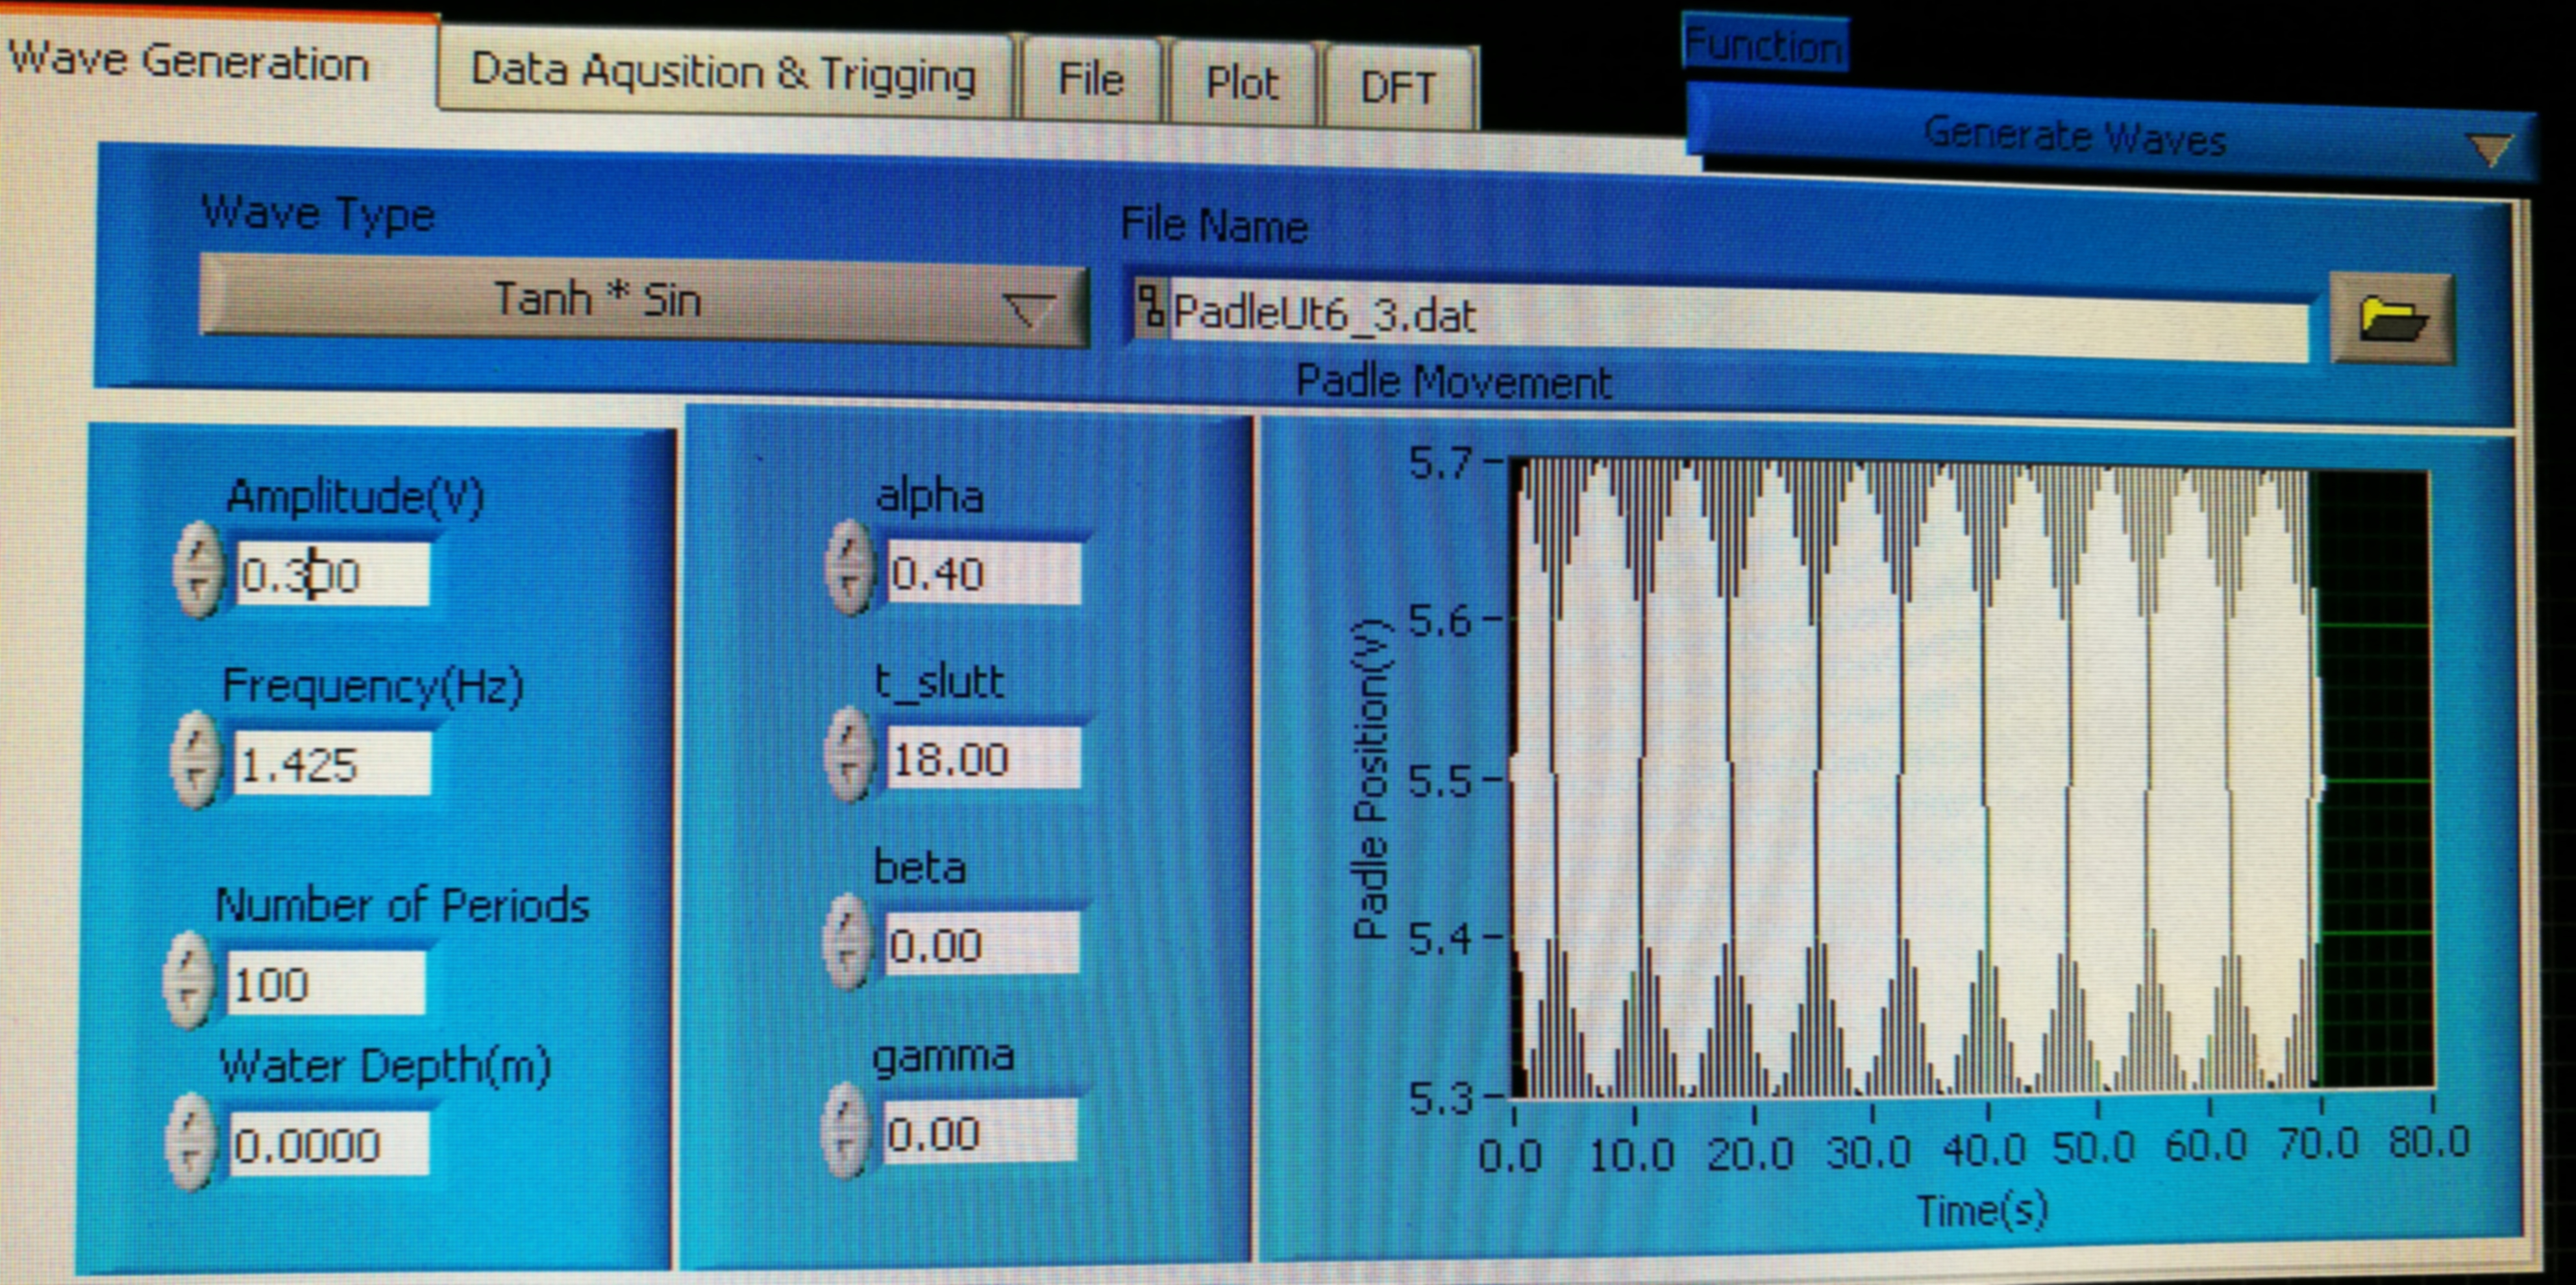
\includegraphics[width=120mm]{wave_maker11.jpg}
    \caption{Image taken of the software that controls the paddle which generates waves in the tank. In this instance the paddle is set to generate high amplitude waves with 0.3V. The frequency was set to 1.425 for all the runs.}
    \label{fig:1}
\end{figure}

For every new wave amplitude, we took another $500$ images three times. After we had run our tests and had gotten images for the four different wave amplitudes, each three times, we selected two images of one crest from all the tests. This gave us $24$ images in total. These were all masked  using 'Gnu Image Manipulation Program', to avoid getting interference from the non essential part of the wave (the wave surface and above). \\ \bigskip

The probes measuring the amplitudes of the waves gave us a lot of data. We found the average of the crest and trough amplitudes and subtracted the trough amplitude by the crest amplitude and divided by two. Since the probes measured the distance from the probe to the water surface, this method would give us the average amplitude of the waves as seen in table \ref{tab:amplitudes}. \\ \bigskip

To find the optimal subwindow sizes, search ranges and overlap percentages, we ran the programs many times and examined plots similar to the ones in figure \ref{fig:4}. All of these plots can be found in the link in the appendix section. We decided upon those that fit the best, and have presented them in the results section.

\section*{Theoretical models}

\begin{table}[H]
    \centering
    \begin{tabular}{|c|c|} \hline
    Important & values \\ \hline \hline
$k$ & 8.17185   \\ \hline
$h$ & 0.72 m \\ \hline
Frequency & 1.425 hz \\ \hline
Gravity acceleration & 9.81 $\text{m/s}^2$ \\ \hline
    \end{tabular}
    \caption{$k$ is the wave number and was found by assuming deep water properties and calculating it by hand. It was also found by not assuming deep water properties and solving the equation, $w^{2} = gk\tanh(hk)$, numerically.
    $h$ is the tank water depth and along with the wave frequency it was given from the beginning. }
    \label{tab:values}
\end{table}

Below we have the most important equations for each of the different types of waves; linear, second order Stokes and third order Stokes. In table \ref{tab:values} we have given that $k = 8.17185$, and this value was found from the second order Stokes wave angular frequency, $\omega^2 = gk$. This formula also holds for linear waves when $kh >> 1$ because then we can set $\tanh(kh) = 1$ in the linear waves angular frequency formula. \\ \bigskip

The value for $k$ was also verified by solving the angular frequency equation for third order Stokes waves and the shallow water angular frequency equation for linear waves numerically. We used Newtons method to find the value for $k$ iteratively. This gave us values ranging from $8.0588$ to $8.18$ depending on which amplitude we used. These are all very close to the analytical value, so we have used $8.172$ in all of our comparisons between the exact and numerical solutions seen in figure \ref{fig:4}.

\begin{table}[H]
    \begin{tabular*}{\textwidth}{c @{\extracolsep{\fill}}c c} 
      & \textbf{Linear waves} ($\theta = kx - wt$)   \\ \hline\\ 
Velocity potential & $\phi = \frac{aw}{k} e^{kz} \sin(\theta)$\\ \hline \\
Horizontal velocity & $u = \frac{\partial \phi}{\partial x} = aw e^{kz}\cos(\theta)$ \\ \hline \\
Vertical velocity & $v = \frac{\partial \phi}{\partial z} = aw  e^{kz}\sin(\theta)$ \\ \hline \\
Surface elevation & $\eta(x,t) = a\cos(\theta)$ \\ \hline \\
Angular frequency & $\omega^{2} = gk\tanh(hk)$ \\ \hline \\
Wave height & $H = 2a$ \\ \hline
    \end{tabular*}
\end{table}

\begin{table}[H]
    \begin{tabular*}{\textwidth}{c @{\extracolsep{\fill}}c c} 
      &\textbf{Second-order Stokes waves}  ($\theta = kx - wt$)  \\ \hline\\ 
Velocity potential & $\phi = \frac{aw}{k} e^{kz} \sin(\theta)$\\ \hline \\
Horizontal velocity & $u = \frac{\partial \phi}{\partial x} = aw e^{kz}\cos(\theta)$ \\ \hline \\
Vertical velocity & $v = \frac{\partial \phi}{\partial z} = aw  e^{kz}\sin(\theta)$\\ \hline \\
Surface elevation & $\eta(x,t) = a(\cos(\theta)+\frac{ka}{2}\cos(2\theta))$\\ \hline \\
Angular frequency & $\omega^{2} = gk$\\ \hline \\
Wave height & $H = 2a + \frac{ka^2}{2}$ \\ \hline
    \end{tabular*}
\end{table}

\begin{table}[H]
    \begin{tabular*}{\textwidth}{c @{\extracolsep{\fill}}c c}
      &\textbf{Third-order Stokes waves}  ($\theta = kx - wt$)  \\ \hline\\ 
Velocity potential & $\phi = \frac{aw}{k} e^{kz} \sin(\theta)$\\ \hline \\
Horizontal velocity & $u = \frac{\partial \phi}{\partial x} = aw e^{kz}\cos(\theta)$ \\ \hline \\
Vertical velocity & $v = \frac{\partial \phi}{\partial z} = aw  e^{kz}\sin(\theta)$\\ \hline \\
Surface elevation & $\eta(x,t) = a(\cos(\theta)+\frac{ka}{2}\cos(2\theta)+\frac{3(ka)^2}{8}\cos(3\theta))$\\ \hline \\
Angular frequency & $\omega^{2} = gk(1+(ka)^2)$\\ \hline \\
Wave height & $H = 2a(1+\frac{3}{8}(ka)^2)$ \\ \hline
    \end{tabular*}
\end{table}

Since we were comparing the horizontal velocity exact solution to the numerical horizontal velocity solution at the crest, we could set $\cos(\theta) = 1$ and get $u=awe^{kz}$ for linear, second order Stokes and third order Stokes waves. The comparisons seen in figure \ref{fig:4} were all made with $u = awe^{kz}$ as the exact solution.


\section*{Results}

\begin{table}[H]
    \centering
    \begin{tabular}{|c|c|c|c|c|} \hline
&       Run 1, 0.05V &       Run 1, 0.1V &  Run 1, 0.2V &     Run 1, 0.3V \\ \hline
Probe 1 &         0.0038  &  0.0064 &      0.0111 &         0.0154 \\ \hline
Probe 2 &         0.0033 &         0.0057 &         0.0101 &         0.0144 \\ \hline
Probe 3 &         0.0037 &         0.006 &  0.0104 &         0.0148 \\ \hline
Probe 4 &         0.0035 &         0.0058 &         0.0102 &         0.0143 \\ \hline \hline
Average &        0.003575 &       0.005975  &      0.01045 &        0.014725 \\ \hline \hline \hline
&        Run 2, 0.05V &       Run 2, 0.1V &        Run 2, 0.2V &        Run 2, 0.3V \\ \hline
Probe 1 &         0.0038 &         0.0063 &         0.0111 &         0.0154 \\ \hline
Probe 2 &         0.0034 &         0.0057 &         0.01 &   0.0144 \\ \hline
Probe 3 &         0.0036 &         0.0059 &         0.0104 &         0.0147 \\ \hline
Probe 4 &         0.0035 &         0.0058 &         0.0101 &         0.0143 \\ \hline \hline
Average &        0.003575 &       0.005925 &       0.0104 &         0.0147 \\ \hline \hline \hline
&       Run 3, 0.05V &       Run 3, 0.1V &        Run 3, 0.2V &        Run 3, 0.3V \\ \hline
Probe 1 &         0.0039 &         0.0063   &  0.0111 &      0.0154 \\ \hline
Probe 2 &         0.0034 &         0.0057   &  0.01 &        0.0144 \\ \hline
Probe 3 &         0.0036 &         0.0059 &         0.0104 &         0.0147 \\ \hline
Probe 4 &         0.0035 &         0.0058   &  0.0102 &      0.0143 \\ \hline \hline
Average &  0.0036 &      0.005925 &      0.010425 &       0.0147 \\ \hline \hline \hline
Average all runs & 0.0036 &      0.006 & 0.0104 &         0.0147 \\ \hline
    \end{tabular}
    \caption{The table shows the average amplitude of each probe for each run and each paddle voltage. It also shows the average over all the probes for each run and also the overall average over all runs for a particular voltage. The table is best read from the top to the bottom, instead of from left to right. This gives you the evolution of the amplitude from run to run.}
    \label{tab:amplitudes}
\end{table}

\begin{table}[H]
    \centering
    \begin{tabular}{|c|c|c|c|c|} \hline
    95\% Confidence & Intervals & for & the & Probes\\ \hline \hline
&      Run 1, 0.05V &       Run 1, 0.1V &  Run 1, 0.2V &     Run 1, 0.3V \\ \hline
Standard Deviation & 3.54e-04 & 4.45e-04 & 7.84e-04 & 8.05e-04 \\ \hline
Lower Bound & 0.0029 & 0.0050 & 0.0089 & 0.0131 \\ \hline
Upper Bound & 0.0043 & 0.0068 & 0.0119 & 0.0163 \\ \hline
    \end{tabular}
    \caption{Here we see the standard deviation between the mean values from each probe. The lower and upper bound of the 95\% confidence interval is then given by $\mu \pm t^*\cdot s$. Here $\mu$ is the mean of the means from each probe, $t^* = 1.960$ from the t-table for $95\%$, and $s$ is the sample standard deviation given by $s=\sqrt{\frac{1}{N-1}\sum_{i=1}^N(\bar{x}-x_i)^2}$.}
    \label{tab:CI}
\end{table}


\begin{figure}[H]
    \centering
    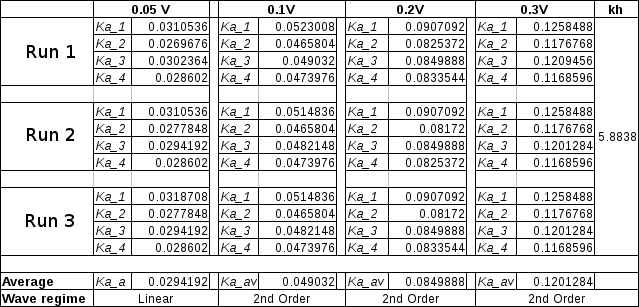
\includegraphics[width=160mm]{snapshot1.png}
    \caption{Here we see the degree of the non-linearity of the waves. $k$ is the wave number and $a$ is the amplitudes from table \ref{tab:amplitudes}, and $k\cdot a$ gives us an indication of the non-linearity. The lower $k\cdot a$ is, the more linear the wave is. Since $k$ is constant $8.172$, the amplitudes dictates the non-linearity.
    In the far right we see  $k\cdot h = 5.8838 >> 1$ which means that we can consider all the experiments as having deep water properties.}
    \label{fig:2}
\end{figure}


\begin{figure}[H]
    \centering
    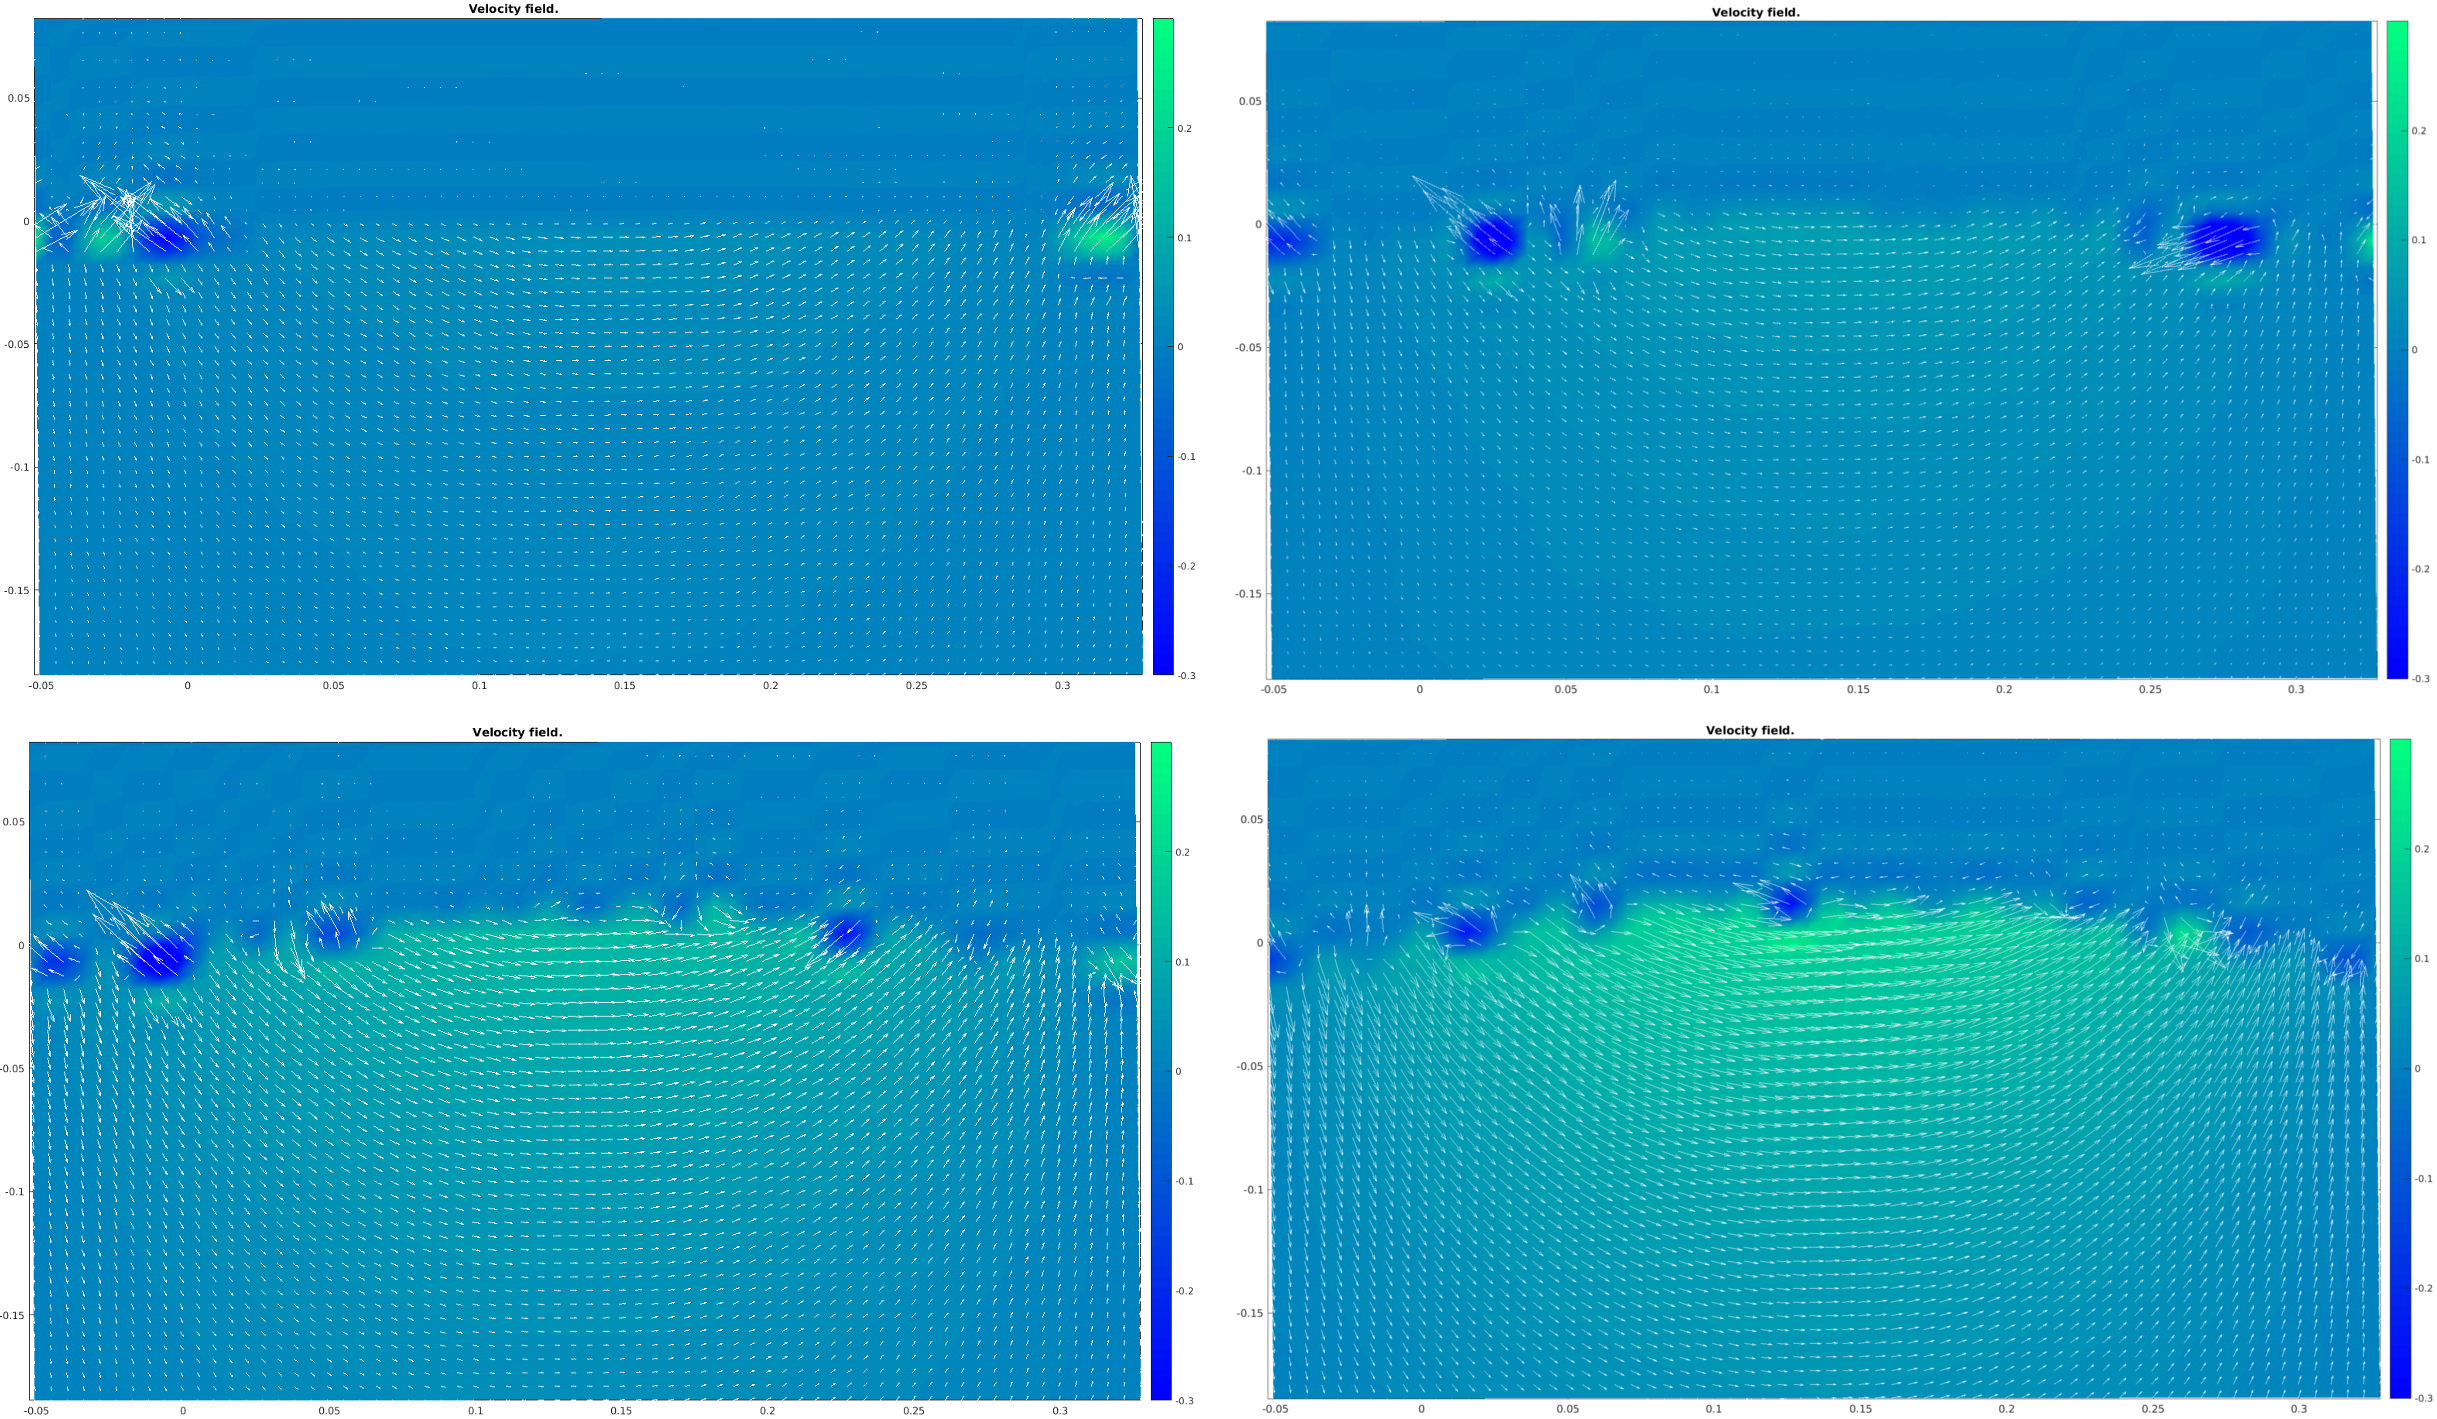
\includegraphics[width=160mm]{Velocity_Field_all_in_one.png}
    \caption{The y- and x-axis are given in meters (m). These are quiver plots of velocity fields from with different amplitudes. The color-bar shows the intensity of the horizontal velocity.
    The top left plot is for 0.05V. The top right plot is for 0.1V. The bottom left plot is for 0.2V. The bottom right plot is for 0.3V.}
    \label{fig:3}
\end{figure}

\begin{figure}[H]
    \centering
    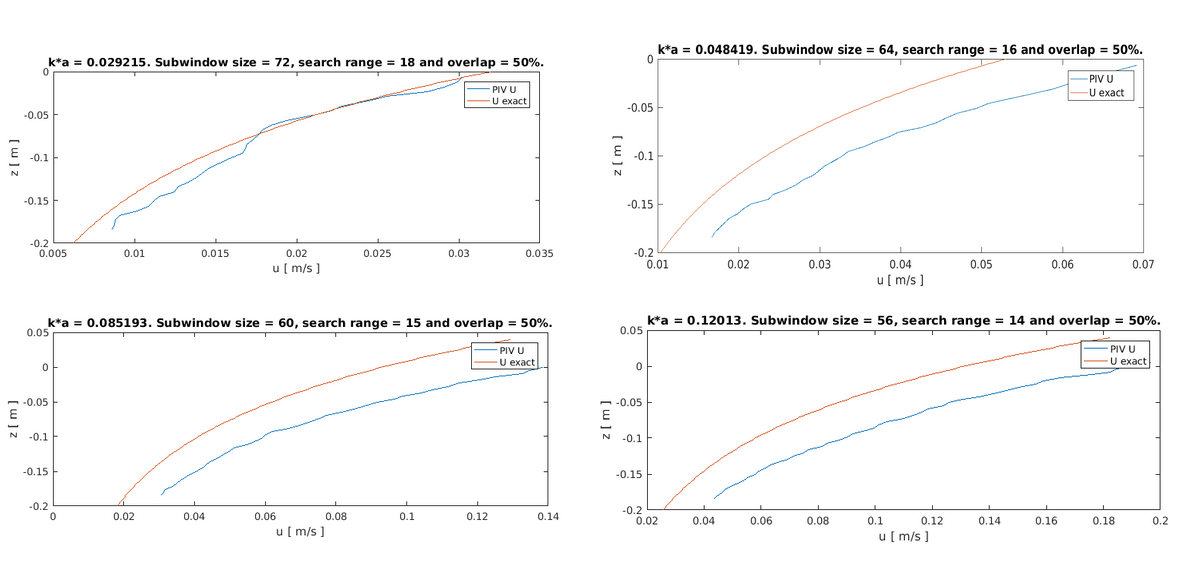
\includegraphics[width=180mm]{velocity_profiles.png}
    \caption{The y-axis is given in meters (m) and the x-axis is given in meter per second (m/s). The red line is the analytical horizontal velocity profile, and the blue line is the numerical horizontal velocity profile found with PIV. The shape of the blue line is very similar to the red line, but it is shifted to the right. This shift indicates that the everything is behaving as it should, but that the numerical horizontal velocity is higher.}
    \label{fig:4}
\end{figure}

\begin{figure}[H]
    \centering
    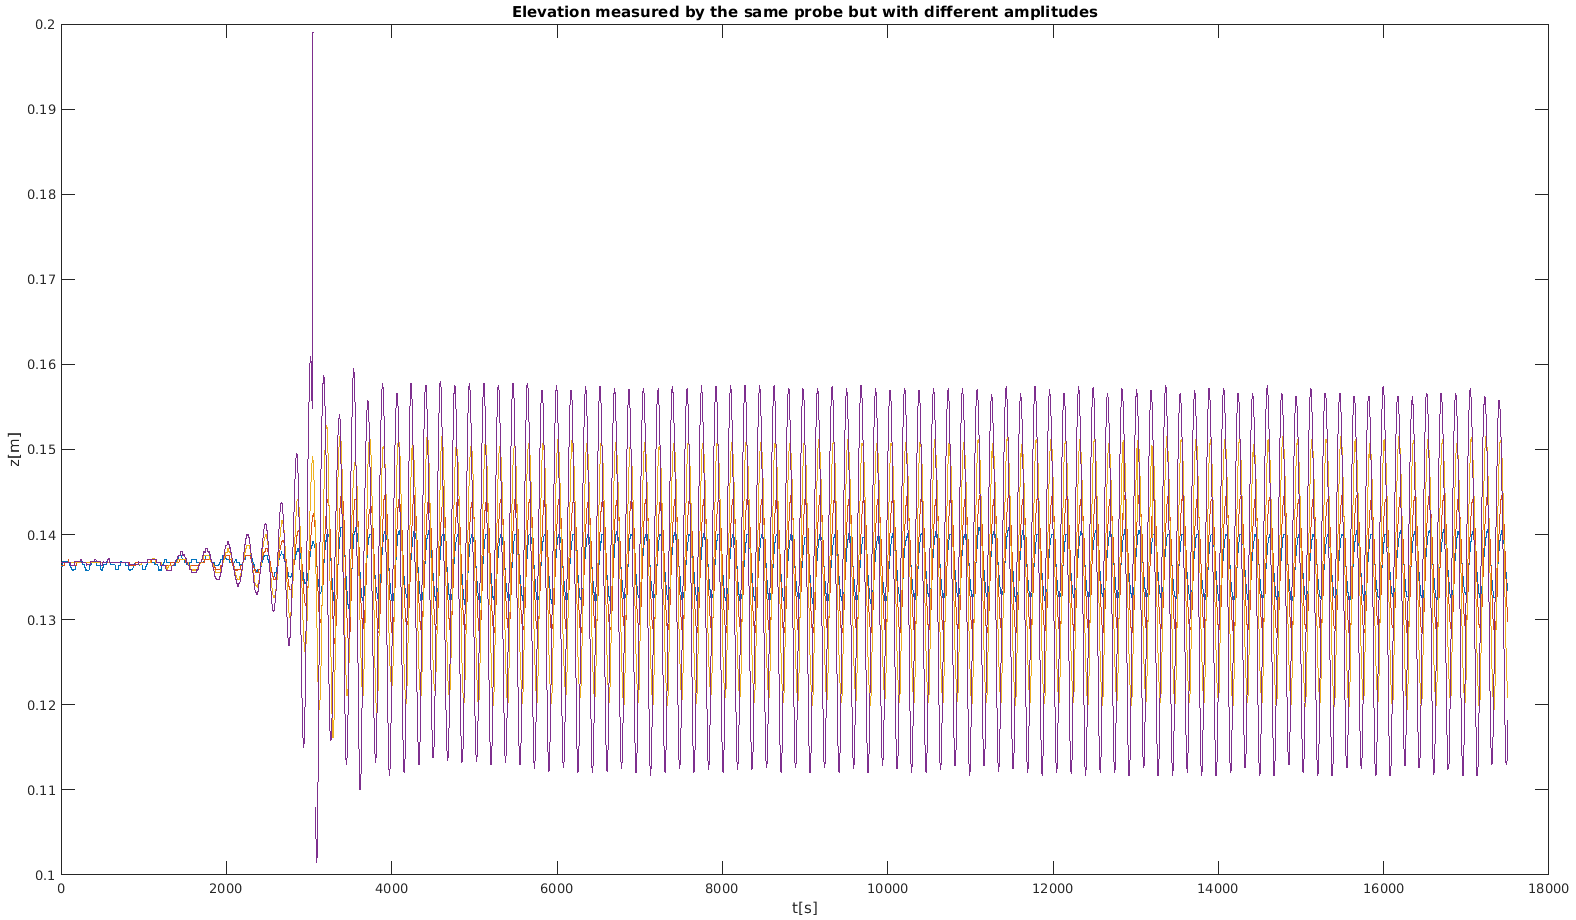
\includegraphics[width=160mm]{B_probe.png}
    \caption{A plot of one of the four probes showing the four different amplitudes. All the other probes show similar behaviour and the plots can be found in the appendix. The y-axis is given in meters (m) and the x-axis numbers every sample the probe takes.}
    \label{fig:5}
\end{figure}

\begin{figure}[H]
    \centering
    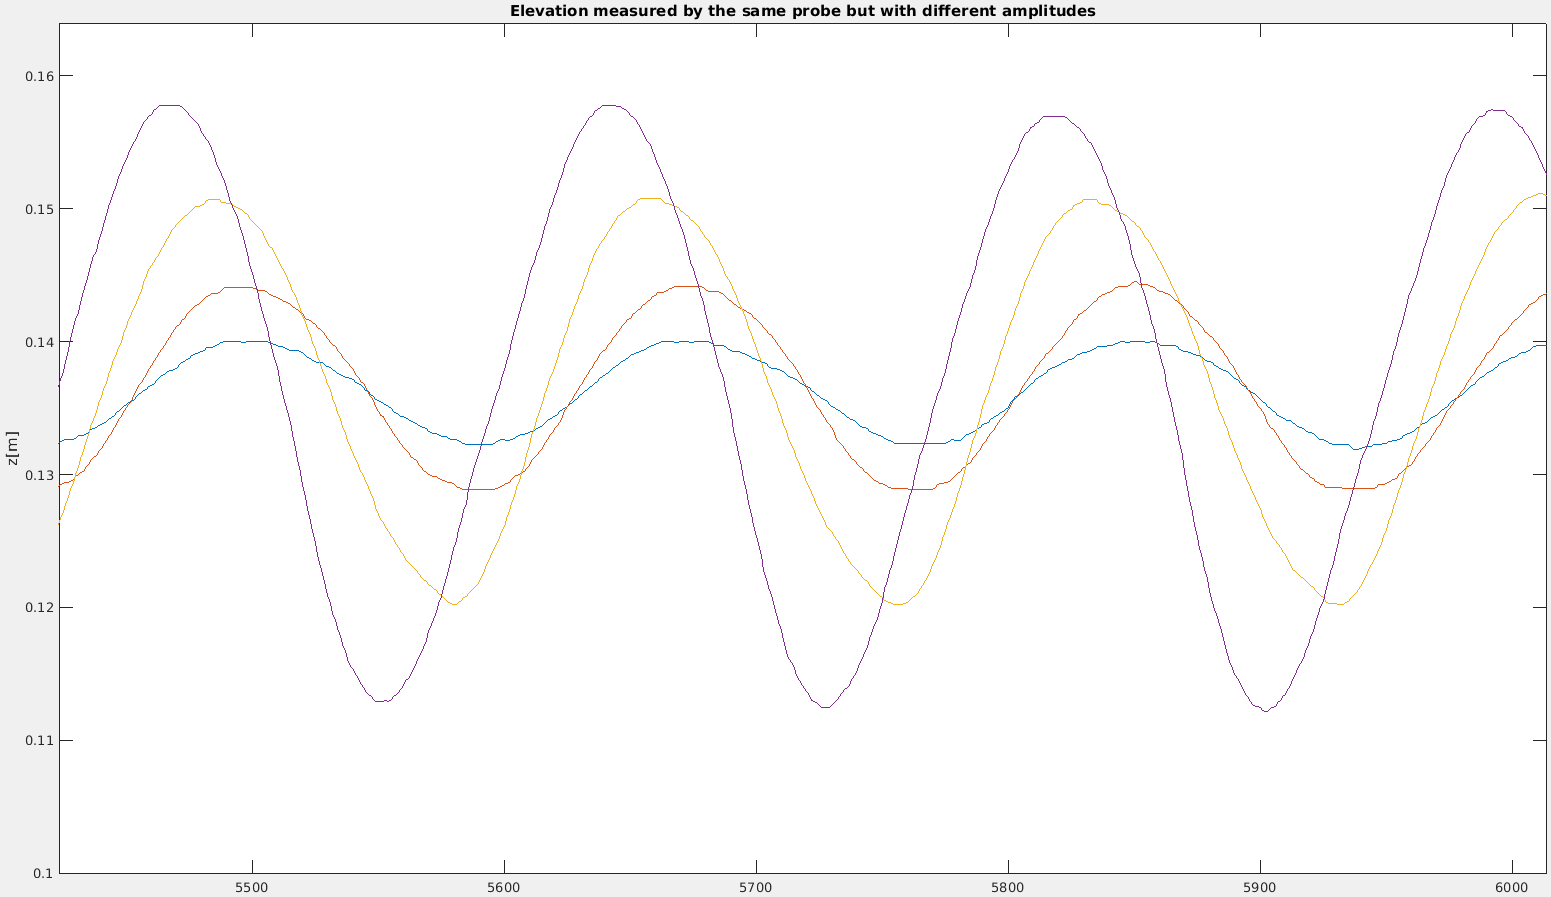
\includegraphics[width=160mm]{B_zoom.png}
    \caption{This is the same as figure \ref{fig:5}, and the only difference is that we have zoomed into a smaller region to see the differences between the different amplitudes. The spacing from crest to crest is consistent between every amplitude, but the higher the amplitude, the more shifted are the crests to the left.}
    \label{fig:6}
\end{figure}


\section*{Discussion}
All of the graphs and numbers are consistent. Figure \ref{fig:3} and figure \ref{fig:4} shows this consistency very well. In figure \ref{fig:3} the color intensity is increasing with the amplitude of the waves, and with the position in the z-axis. We see that the green color is the most intense in the middle and around the top of the wave. This is consistent with what we see in figure \ref{fig:4} which shows that the highest horizontal velocities are close to the top of the wave. \\ \bigskip

While the blue lines in figure \ref{fig:4} is a bit off, the overall shape is very similar to the red line, which is the exact solution. The reason to why the blue line is a bit off may be due to seeding issues, not enough or too much. \\ \bigskip

A very curious discovery is the fact that the amplitudes are consistently shifted to the left in figure \ref{fig:6}. This shifting is not seen in figure \ref{fig:5}, but when zoomed in, it is very clear to see. Why this is happening, is not known to us. But since the spacing from crest to crest is the same always, there is nothing to worry about.\\ \bigskip

The Stokes waves have higher troughs and crests than linear waves as seen in figure \ref{fig:stokes} below, and therefore table \ref{tab:amplitudes} might have some errors. How substantial this error is, is uncertain.

\begin{figure}[H]
    \centering
    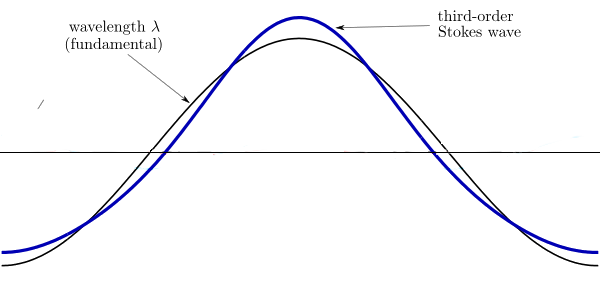
\includegraphics[width=100mm]{stokes1.png}
    \caption{This graph shows the different between linear waves and Stokes waves. The Stokes waves are much sharper and are somewhat elevated above the linear waves.}
    \label{fig:stokes}
\end{figure}

From table \ref{tab:CI} we can see that the standard deviation doubles from 0.05V to 0.3V. This increase may also be connected to the fact that third order Stokes waves are elevated above linear waves. But it might also be connected to the fact that there is more and more disturbances at the surface when looking at the quiver plots in figure \ref{fig:3}. There is no substantial proof for this, and the surface disturbances may simply be due to bad masking where too much of the surface is still visible. \\ \bigskip

\section*{Conclusion}
To us the 0.3V waves with high amplitude looked more like linear waves, but to our surprise only the waves with very low amplitude was behaving linearly. These waves were very small to us, as can be seen in figure \ref{fig:3}, and learning about how fast waves become non linear was great. \\ \bigskip

Surprisingly all of our data seemed very in line with the theoretical models. Of course the numerical data was not perfect as seen in figure \ref{fig:4}, but the similarities were striking. To be able to create such well behaved waves and gather so much information from them was absolutely great. \\ \bigskip

This project was huge and we had to learn a lot of new things very quickly. While the introduction to the HydroLabPIV software in the previous project was a tremendous help, we still had a lot to do. We had to redo all of our measurements in the lab because we had a suspicion that our data was corrupted due to reflection waves.\\ \bigskip

We had to be very careful to not jump to any conclusions with a good reason or evidence for doing so. This was a challenge because it meant we had to run a lot of code, sift through a lot of data and read a lot of theory to try to find answers to subwindow sizes, search ranges, amplitudes, equations and more. It sure was a challenging project.


\section*{Appendix}
For matlab code, images and tex source code, see the link below:

\url{https://github.com/ShakoFarhad/PIV-Project-2}

\bibliographystyle{plainnat}
\bibliography{mybib} \bigskip \bigskip
\end{document}
